% Document information
\newcommand{\titleinfo}{Zusammenfassung OO-Analyse und -Design}
\newcommand{\authorinfo}{Sandro Pedrett}
\newcommand{\version}{1.0}
\newcommand{\versioninfo}{FS22}
% Header
\include{Template/Header}

% Setup Source Code
\lstset{ 
	backgroundcolor=\color{white},   % choose the background color; you must add \usepackage{color} or \usepackage{xcolor}; should come as last argument
	basicstyle=\footnotesize,        % the size of the fonts that are used for the code
	breakatwhitespace=true,         % sets if automatic breaks should only happen at whitespace
	breaklines=true,                 % sets automatic line breaking
	captionpos=b,                    % sets the caption-position to bottom
	commentstyle=\color{ForestGreen},    % comment style
	escapeinside={\%*}{*)},          % if you want to add LaTeX within your code
	extendedchars=true,              % lets you use non-ASCII characters; for 8-bits encodings only, does not work with UTF-8
	frame=single,	                   % adds a frame around the code
	keepspaces=true,                 % keeps spaces in text, useful for keeping indentation of code (possibly needs columns=flexible)
	language=c,                      % the language of the code
	numbersep=5pt,                   % how far the line-numbers are from the code
	rulecolor=\color{black},         % if not set, the frame-color may be changed on line-breaks within not-black text (e.g. comments (green here))
	showspaces=false,                % show spaces everywhere adding particular underscores; it overrides 'showstringspaces'
	showstringspaces=false,          % underline spaces within strings only
	showtabs=false,                  % show tabs within strings adding particular underscores
	stepnumber=2,                    % the step between two line-numbers. If it's 1, each line will be numbered
	tabsize=2,	                   % sets default tabsize to 2 spaces
	title=\lstname,                   % show the filename of files included with \lstinputlisting; also try caption instead of title
	stringstyle=\ttfamily\color{red!50!brown},
	keywordstyle=\color{blue}\bfseries,
}

% open-book

% Document
\begin{document}

\tableofcontents 
\newpage

\section{Einführung}
Ziel der OOA (Analyse) ist es, die Wünsche und Anforderungen des Auftraggebers zu erfassen und beschreiben. OOA ist technologie unabhängig und entählt keine Optimierungen. Objektorientierung hilft dabei, komplexe System mit angemessenen Mitteln zu dokumentieren, da diese Konzept gut auf die Reelle Welt überführt werden kann. Zur Visualisierung wird oft eine Programmiersprachen-unabhängiges Diagram 'UML' (Unified Modeling Language) verwendet.\\
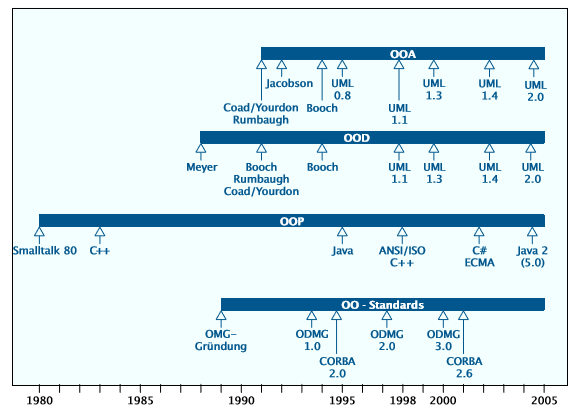
\includegraphics[width=\columnwidth]{Images/geschichte}


OOD (Design) ist die Vorstufe der Implementierung und verfeinert die OOA mit Deteils. Die Architektur zusammen Optimierungen und Technologien werden hier festgelegt.

\textbf{tl:dr} OOA sagt \textit{was} das System können muss, OOD sagt \textit{wie} das System das das macht. \newpage
\section{UML Notation}
\subsection{Klassendiagramm}
Das statische Klassendiagramm beschreibt die Verbindungen zwischen einzelnen Klassen und Generalisierungen.
\begin{center}
	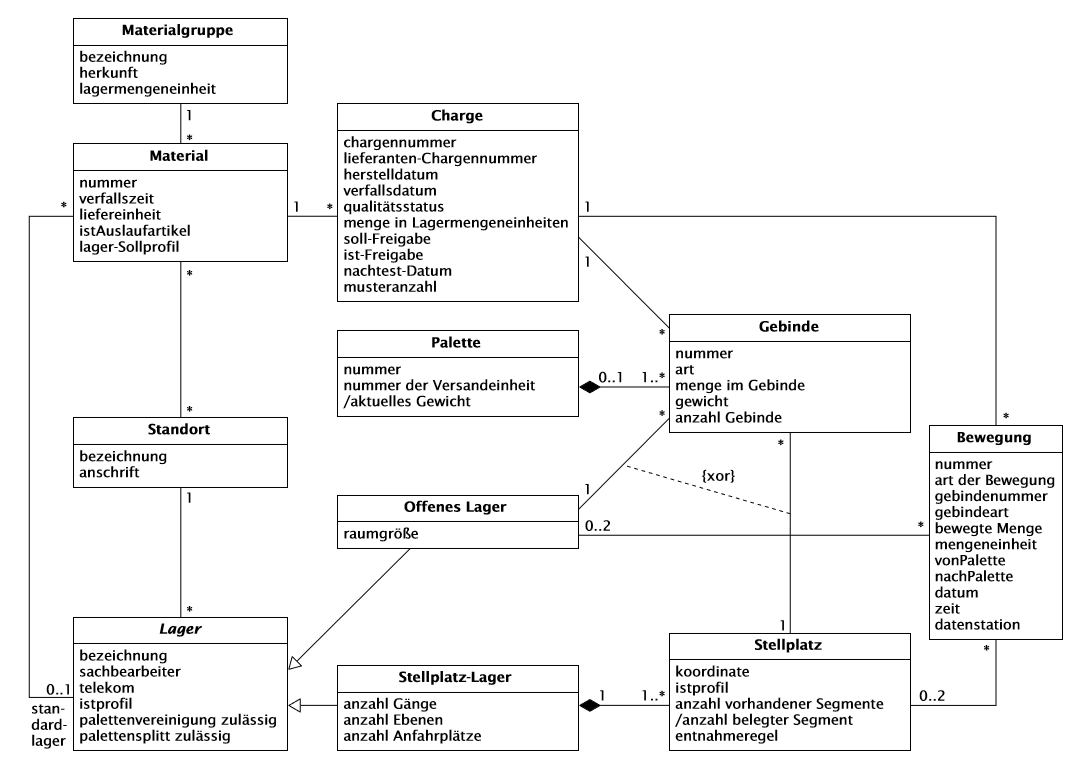
\includegraphics[width=\columnwidth]{Images/klassendiagramm}
\end{center}

\subsubsection{Klasse}
Die Klasse ist eine Vorlage für ein beliebiges Objekt. Klassennamen sind Substantiv im Singular, das durch ein Adjektiv ergänzt werden kann.
\begin{center}
	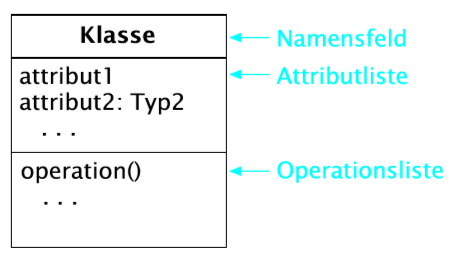
\includegraphics[width=0.4\columnwidth]{Images/class}
\end{center}
\textbf{Attribute} sind wie folgt definiert:
\begin{lstlisting}
sichtbarkeit name: type ('{' Eigenschaft '}' | '=' Anfangswert | '[' Range ']')?
\end{lstlisting}Sichtbarkeiten:
\begin{itemize}[nosep]
	\item + öffentlich
	\item - privat
	\item \# geschützt
	\item / abgeleitet
	\item \~\ Paket
	\item * zufällig
\end{itemize}~\\

\subsubsection{Assoziation}
Assoziationen verbinden Klassen miteinander.
\begin{center}
	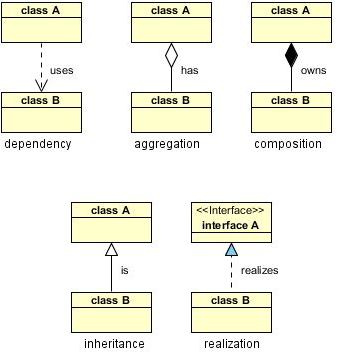
\includegraphics[width=0.6\columnwidth]{Images/assoziation}
\end{center}


\textbf{Lesen}\\
Verbindungen werden wie folgt gelesen:
Artikel (1) hat beliebige (2) Auftragspositionen (3).\\
\begin{center}
	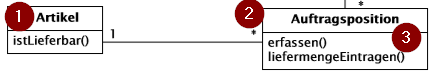
\includegraphics[width=0.8\columnwidth]{Images/lesen}
\end{center}

\textbf{Beispiel}\\
\begin{center}
	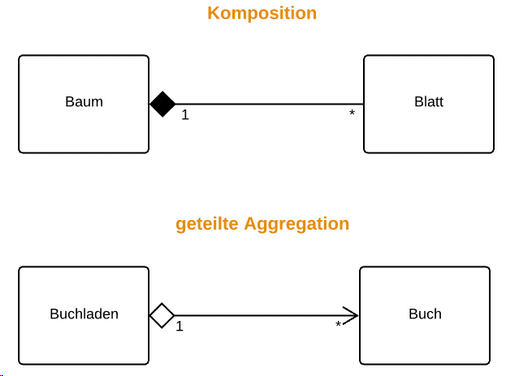
\includegraphics[width=0.6\columnwidth]{Images/assoziation2}
\end{center}

\textbf{Multiplizität}\\
Zu einer Multiplizität kann auch ein Rollenname, welche die Assoziation beschreibt, hinzugefügt werden.
\begin{center}
	\includegraphics[width=0.6\columnwidth]{Images/multiplizität}
\end{center}

\textbf{Eigenschaften}\\
\textit{ordered} oder \textit{subsets} können zusätzlich zu der Assozation hinzugefügt werden, um weitere Einschränkungen zu beschreiben\\

\textbf{Assoziationsklasse}\\
Eine Assoziationsklasse besitzt Eigenschaften einer Klasse. Im Design-Prozess muss diese meistens in eine Klasse transformiert werden.
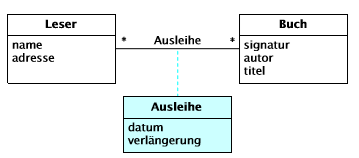
\includegraphics[width=\columnwidth]{Images/assoziationsklasse}\\

\textbf{Abgeleitet Assoziation}\\
Wenn Assoziationen doppelt vorhanden sind,  werden diese mit einem '/' gekennzeichnet.\\

\textbf{Navigierbarkeit}\\
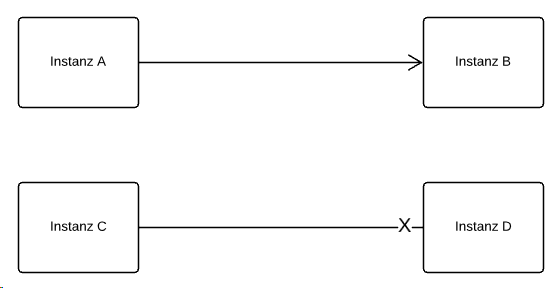
\includegraphics[width=\columnwidth]{Images/navigierbarkeit}
Instanz B erreichbar für Instanz A und Instanz D nicht erreichbar für Instanz C. Falls keine Navigierbarkeit benötigt wird, keine Notation.

\textbf{Generalisierung}\\
\begin{center}
	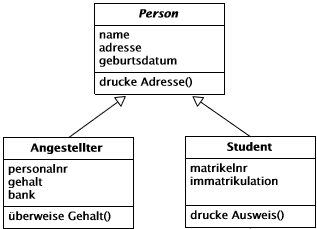
\includegraphics[width=0.5\columnwidth]{Images/generalisierung}
\end{center}


\subsection{Use-Case}
Use-Case beschreiben, was ein Akteur von einem System erwarten kann. 
\begin{center}
	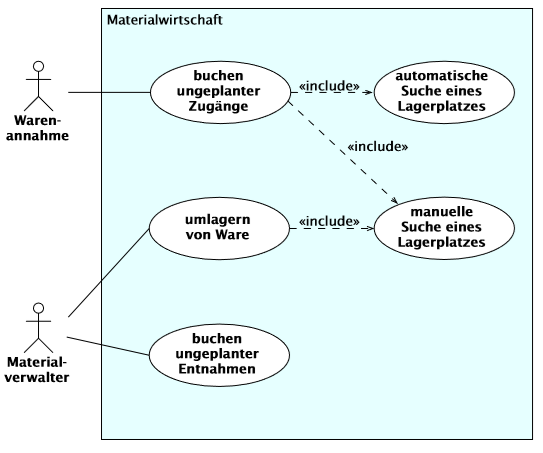
\includegraphics[width=\columnwidth]{Images/usecase}
\end{center}

\subsubsection{Extension}
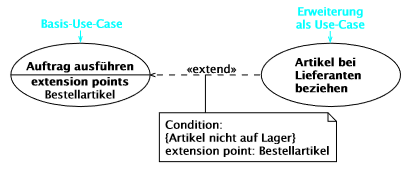
\includegraphics[width=\columnwidth]{Images/extension}

\subsection{Aktivitäten}
Das Aktivitäten-Diagramm beschreibt den dynamischen Ablauf eines Prozesses.\\
\includegraphics[width=\columnwidth]{Images/Aktivitätendiagramm}


\subsubsection{Knoten}
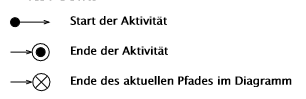
\includegraphics[width=0.6\columnwidth]{Images/knoten}

\subsubsection{Splitting}
Events welche unabhängig (Nebenläufig) ausgeführt werden können, können durch Splitting geteilt und zusammengeführt werden.\\
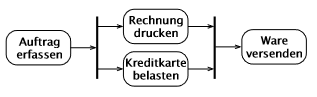
\includegraphics[width=0.6\columnwidth]{Images/splitting}


\subsubsection{Schwimmbahnen}
Zu den Aktivitäten können zusätzliche Pakete (in c++ sind diese Namespaces) hinzugefügt werden.\\
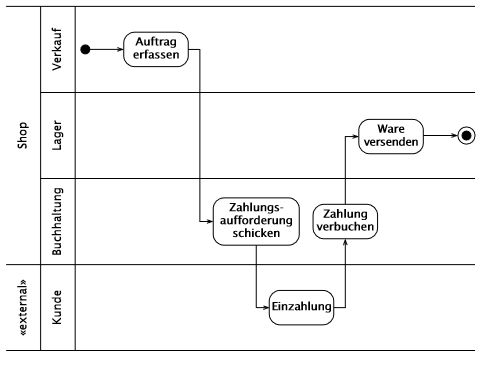
\includegraphics[width=\columnwidth]{Images/schwimmbahnen}

\subsection{Szenario}
Ein Szenario ist eine Sequenz von Verarbeitungsschritten, die unter bestimmten Bedingungen auszuführen ist. Im Gegensatz zu einem Use-Case, welche eine Sammlung von Szenarien ist, beschreibt das Szenario-Diagramm nur ein möglichen Fall.
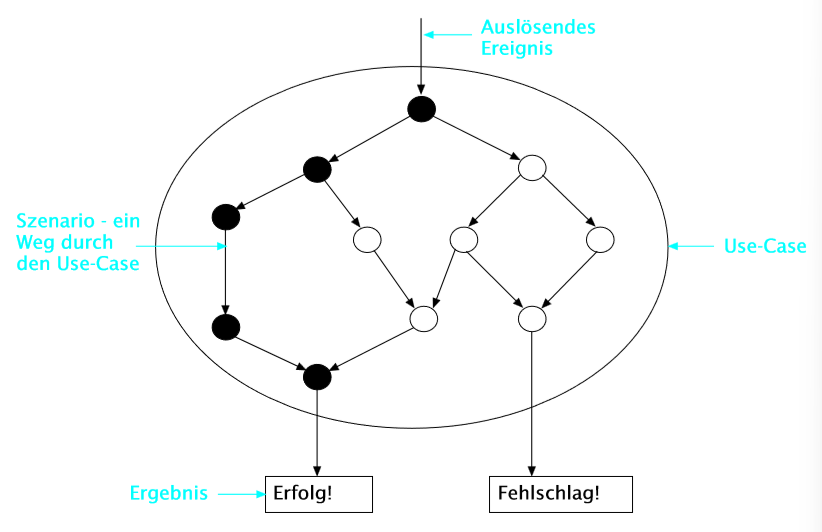
\includegraphics[width=\columnwidth]{Images/szenario}


\subsection{Sequenzdiagramm}
Sequenzdiagramm zeigt die Kommunikation zwischen mehreren Kommunikationspartnern, wobei jeder Parnter (Lebenslinie) durch Rechteck und vertikale gestrichelte Linie dargestellt wird. Das Diagramm besitzt zwei Dimensionen, Zeit vertikal, Kommunikationspartner Horizontal. Return-Werte können mit Pfeil oder mit Doppelpunkt Notation definiert werden.
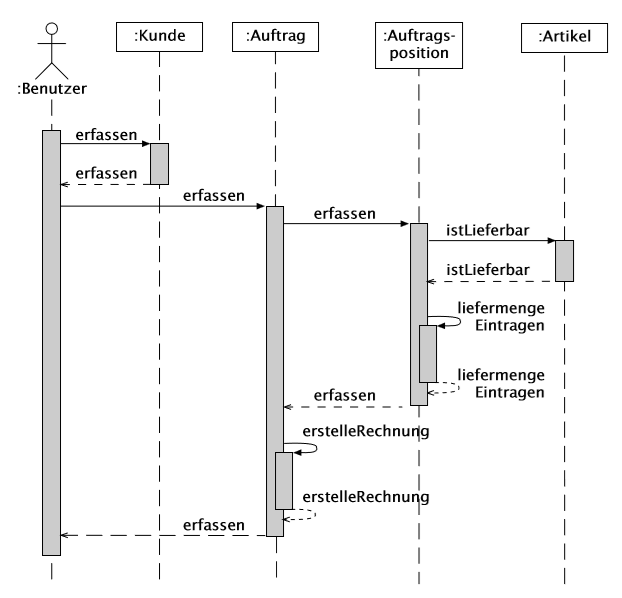
\includegraphics[width=\columnwidth]{Images/sequenzdiagramm}

\subsubsection{Nachrichten}
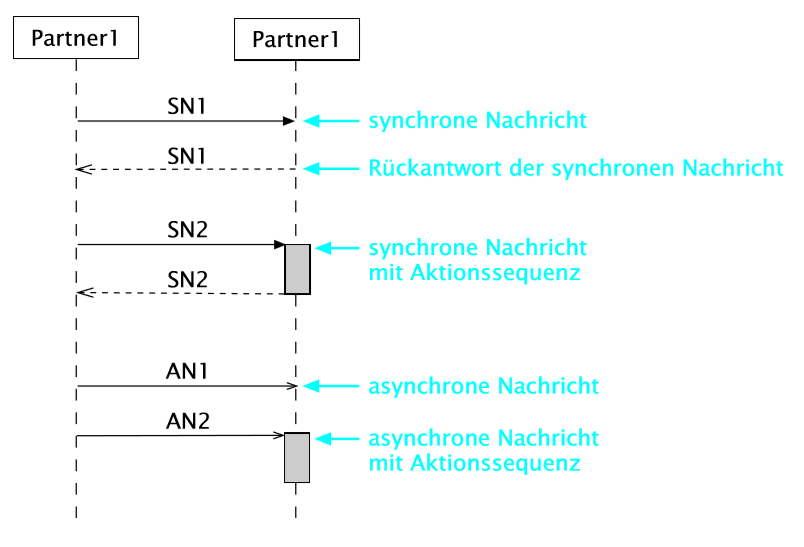
\includegraphics[width=\columnwidth]{Images/nachrichten}

\subsection{Kommunikationsdiagramm}
Ist gut geeignet, um das grundsätzliche Zusammenspiel mehrerer Partnern zu zeigen. Schleifen und Bedingungen können einfacher modelliert werden. Ist ähnlich zu Sequenzdiagramm, jedoch ist die Zeit nicht auf einer Achse fixiert.\\

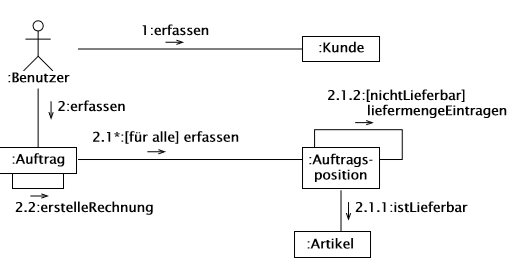
\includegraphics[width=\columnwidth]{Images/kommunikationsdiagramm}
Wichtig ist, dass jeder Verlauf nummieriert ist. Wenn mehrer Verzweigungen möglich sind, etappe tiefer nummerieren.

\subsection{Zustandsautomat}
Jede Transition wird durch ein Ereignis ausgelöst.
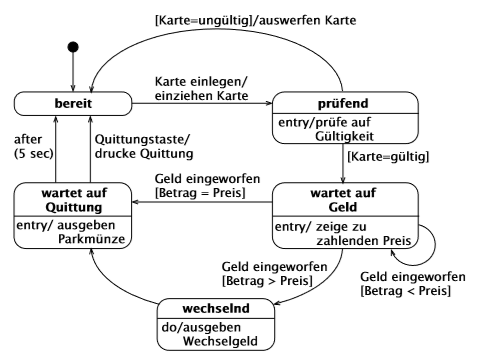
\includegraphics[width=\columnwidth]{Images/zustandautomat}

\textbf{Aktivität}:\\ Es gibt \textit{entry}, \textit{exit} und \textit{do} Zustand.
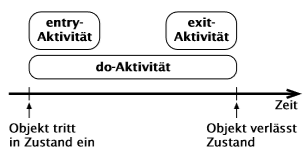
\includegraphics[width=0.4\columnwidth]{Images/aktivität}

\textbf{Protokoll}\\ Ist einer Klasse zugeordnet. Es beschreibt welche Operationen in welchem Zustand aufgerufen werden dürfen.
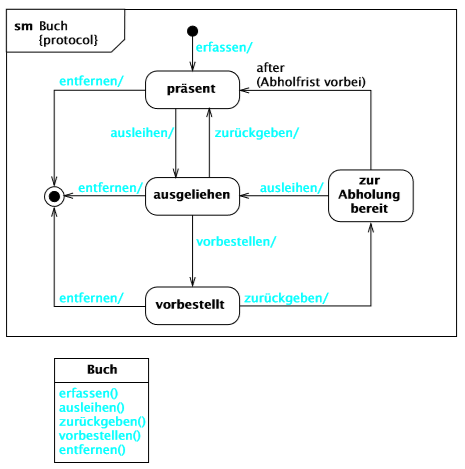
\includegraphics[width=\columnwidth]{Images/protokoll}

\section{OO-Design}
\subsection{Schnittstellen}
Zwei Möglichkeiten Schnittstellen darzustellen. Erstes wird vorallem von High-Level Architekten verwendet.\\
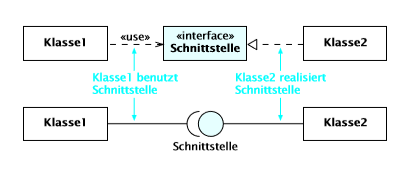
\includegraphics[width=\columnwidth]{Images/schnitstellen}
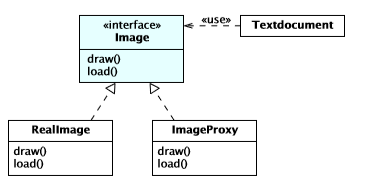
\includegraphics[width=\columnwidth]{Images/schnittstelle_beispiel}

\subsection{Komponenten Diagramm}
\begin{center}
	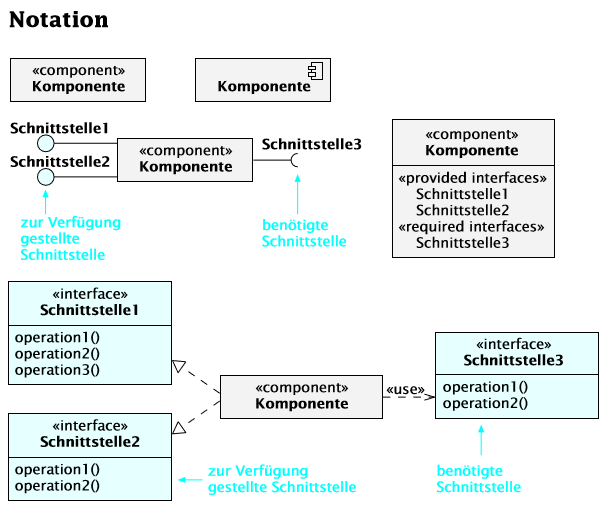
\includegraphics[width=0.9\columnwidth]{Images/komponentdiagramm}
\end{center}

Artefakte enthalten physische Informationen zB Dateien, Executable etc. Abhängigkeiten werden wie folgt definiert:
\begin{center}
	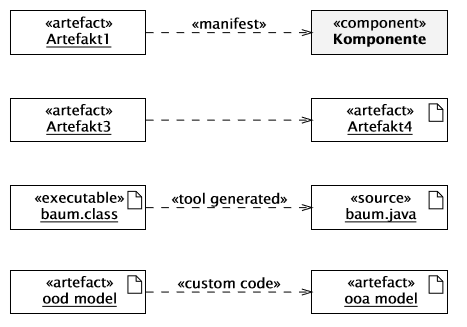
\includegraphics[width=\columnwidth]{Images/artefakte}
\end{center}



\end{document}